\documentclass[a4paper]{article}
\usepackage[UTF8]{ctex}
\usepackage{geometry}
\usepackage{graphicx}
\usepackage{url}
\usepackage{multirow}
\usepackage{array}
\usepackage{booktabs}
\usepackage{url}
\usepackage{enumitem}
\usepackage{graphicx}
\usepackage{float}
\usepackage{amssymb}
\usepackage{amsmath}
\usepackage{subfig}
\usepackage{longtable}
\usepackage{color}

\geometry{a4paper, scale=0.78}

\title{Linear Classification 02}
\author{Chen Gong}
\date{30 October 2019}

% \begin{figure}[H]
%     \centering
%     \includegraphics[width=.55\textwidth]{E.png}
%     \caption{矩阵与列向量的乘法}
%     \label{fig:my_label_1}
% \end{figure}

% \left\{
% \begin{array}{ll}
%       x+2x+z=2 & \\
%       3x+8y+z=12 & \\
%       4y+z=2
% \end{array}
% \right.

\begin{document}

\maketitle
本节的主要内容是描述两类硬分类模型,也就是感知机模型和线性判别模型(Fisher判别模型)的算法原理和推导过程。

\section{感知机模型}
感知机模型是一类错误驱动的模型,它的中心思想也就是"错误驱动"。什么意思呢?也就是哪些数据点分类错误了,那么我们就进行调整权值系数$w$,直到分类正确为止。

\begin{figure}[H]
    \centering
    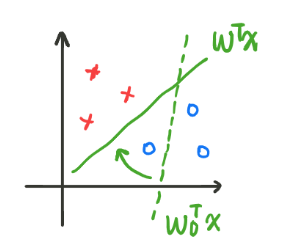
\includegraphics[width=.4\textwidth]{微信图片_20191030090710.png}
    \caption{感知机概念模型图}
    \label{fig:my_label_1}
\end{figure}

感知机可以做如下的描述:
\begin{gather}
    f(x)=sign\{ w^Tx \} \quad x\in \mathbb{R}^p \ w\in  \mathbb{R}^p \\
    sign(a)=
    \left\{
    \begin{array}{ll}
      +1 & a \geq 0 \\
      -1 & a < 0 \\
    \end{array}
    \right.
\end{gather}
其中$D:\{$ 被错误分类的样本 $\}$,样本集为:$\{(x_i,y_i)\}_{i=1}^N$。

\subsection{感知机模型的迭代过程}
我们将损失函数定义为:
\begin{equation}
    \mathcal{L}(w)=\sum_{i=1}^NI\left\{ y_iw^Tx_i < 0 \right\}
\end{equation}

而其中$y_iw^Tx_i < 0$就代表分类错误的类,为什么这么理解呢?因为:
\begin{equation}
    \left\{
    \begin{array}{ll}
      w^Tx_i \geq 0 & y_i=+1 \\
      w^Tx_i < 0 & y_i=-1 \\
    \end{array}
    \right.
\end{equation}
那么当分类正确时,必然有$w^Tx_iy_i>0$。只有当错误分类的时候,才会出现$w^Tx_iy_i<0$的情况。而在上述的函数中,$I$干了一个什么事,那就是将函数的值离散化,令$\mathcal{L}$的值等于错误分类的点的个数,也就是这样一个映射$I\mapsto0,1$。加这个函数的目的是得到损失函数的值,和普通的梯度下降法的过程一样。显然这不是一个连续的函数,无法求得其梯度来进行迭代更新。那么,我们需要想的办法是将离散的梯度连续。那么,我们将损失函数改写为:
\begin{equation}
    \mathcal{L}(w)=\sum_{x_i\in D}-y_iw^Tx_i
\end{equation}

那么,梯度可以表示为:
\begin{equation}
    \nabla_{w}\mathcal{L} = -\sum_{x_i\in D}y_ix_i
\end{equation}

很显然,有关于$w$的迭代公式,可以表示为:
\begin{equation}
    w^{(t+1)}\longleftrightarrow w^{(t)}-\lambda \nabla_w L
\end{equation}

代入可得,权值参数$w$的更新过程为:
\begin{equation}
    w^{(t+1)}\longleftrightarrow w^{(t)}+\lambda \sum_{x_i\in D}y_ix_i
\end{equation}

那么,通过上述的推导,我们就得到了感知机中$w$的更新过程。那么,感知机算法的推导过程就已经完成了。


\end{document}
